\documentclass[amsmath,superscriptaddress,showpacs,aps,prl,onecolumn,notitlepage]{revtex4-1}
\usepackage[colorlinks,linkcolor=blue,anchorcolor=blue,citecolor=blue,urlcolor=blue]{hyperref}
\usepackage{amsmath}
\usepackage{amssymb}
\usepackage{graphicx}
\usepackage{color}
\usepackage{bm}

\begin{document}
\title{Thermal Hall conductivity of flatband itinerant ferromagnets}
\author{Zhao-Long Gu}
\affiliation{National Laboratory of Solid State Microstructures and Department of Physics, Nanjing University, Nanjing 210093, China}
\author{Zhao-Yang Dong}
\affiliation{Department of Applied Physics, Nanjing University of Science and Technology, Nanjing 210094, China.}
\affiliation{National Laboratory of Solid State Microstructures and Department of Physics, Nanjing University, Nanjing 210093, China}
\author{Shun-Li Yu}
\affiliation{National Laboratory of Solid State Microstructures and Department of Physics, Nanjing University, Nanjing 210093, China}
\affiliation{Collaborative Innovation Center of Advanced Microstructures, Nanjing University, Nanjing 210093, China}
\author{Zi-Qiang Wang}
\affiliation{Department of Physics, Boston College, Chestnut Hill, Massachusetts 02467, USA}
\author{Jian-Xin Li}
\email[]{jxli@nju.edu.cn}
\affiliation{National Laboratory of Solid State Microstructures and Department of Physics, Nanjing University, Nanjing 210093, China}
\affiliation{Collaborative Innovation Center of Advanced Microstructures, Nanjing University, Nanjing 210093, China}
\date{\today}


\maketitle
%\widetext
%\newpage
\appendix
%\section{Supplemental Material}

\setcounter{equation}{0}
\setcounter{figure}{0}
\setcounter{table}{0}
\setcounter{section}{0}
\renewcommand{\theequation}{S\arabic{equation}}
\renewcommand{\thesection}{S\arabic{section}}
\renewcommand{\thetable}{S\arabic{table}}
\renewcommand{\thefigure}{S\arabic{figure}}

\par In local spin models, the thermal Hall conductivity $\kappa_{xy}$ of magnons can be computed by the following formula proposed in Ref. \cite{Matsumoto_PRB2014} in the framework of linear spin wave theory:
\begin{equation}\label{THC}
\kappa_{xy}=-\frac{k_B^2T}{\hbar V}\sum_{\mathbf{k}}\sum_{n=1}^N\left\{c_2\left[g(\epsilon_{n\mathbf{k}})\right]-\frac{\pi^2}{3}\right\}\Omega_{n\mathbf{k}}
\end{equation}
Here, $k_B$ is the Boltzmann constant, $\hbar$ is the reduced Planck constant, $T$ is the temperature, $V$ is the system volume, $N$ is the number of spin wave branches, $\epsilon_{n\mathbf{k}}$ is the eigenenergy of the magnon with momentum $\mathbf{k}$ in the $n$th branch, $g$ is the Bose-Einstein distribution function, $\Omega_{n\mathbf{k}}$ is the Berry curvature of the $n$th spin wave branch at momentum $\mathbf{k}$, and the function $c_2(x)$ is defined as follows:
\begin{equation}\label{C2}
c_2(x)\equiv\int_0^xdt\left(\ln\frac{1+t}{t}\right)^2=(1+x)\left(\ln\frac{1+x}{x}\right)^2-(\ln x)^2-2\text{Li}_2(-x)
\end{equation}
where $\text{Li}_2(x)$ is a polylogarithm function $\text{Li}_n(x)$ for $n=2$. It is noted that each Bloch eigenstate of the magnons contributes to the thermal Hall conductivity by a portion that is the product of its Berry curvature and the function $c_2\left[g(\epsilon_{n\mathbf{k}})\right]-\frac{\pi^2}{3}$. The coefficient $-\frac{\pi^2}{3}$ in this function can be neglected for lattice models because in this situation the Berry curvature of all spin wave branches sums to zero.

\par For the case of itinerant magnets, the calculation of thermal Hall conductivity turns out to be more complicated. On the one hand, itinerant magnons, as the bound states of spin-1 particle-hole excitations, are not canonical bosons. Therefore, strictly speaking, they do not obey the Bose-Einstein distribution. While, to get the thermal dynamic quantities, such as the thermal Hall conductivity, multi-magnon excitations must be considered. In itinerant magnets, the exact treatment is beyond the computational capacity. A reasonable way out of this dilemma is to approximate the itinerant magnons as canonical bosons, then Eq. (\ref{THC}) would apply. One the other hand, in magnetically ordered itinerant electronic systems, in addition to the magnons, there also exist Stoner modes, which are individual spin-1 particle-hole excitations. In principle, Stoner modes should contribute to the thermal Hall conductivity as well. Yet no study has been found as to how they contribute to it. Fortunately, Stoner modes usually appear in the high-energy part of the spin-1 excitations and could be neglected when only low-temperature thermal Hall conductivity is focused. Another tricky point resulting from the Stoner modes is their couplings to the optical magnonic band, making the Berry curvature there ill-defined. Therefore, a reliable determination of the contribution to the thermal Hall conductivity from the optical magnonic band persists to be unclear. When the optical band is separated by a large enough energy gap from the acoustic band, such contributions could also be ignored when the temperature is low compared to the bandwidth of the magnons. This condition restricts the model parameter range and temperature range where we could reasonably calculate the thermal Hall conductivity in itinerant magnets by Eq. (\ref{THC}).

\par In the top panels of Fig. \ref{THWT}, we show the temperature dependence of the thermal Hall conductivity for three topologically different phases in the temperature range which is far below the energy of the acoustic band top. The model parameters are such chosen that the optical band is well separated from the acoustic band by an energy gap, as can be seen in the central panels of Fig. \ref{THWT}. So, the contributions from the acoustic band dominate. The Berry curvature $\Omega_{n\mathbf{k}}$ in Eq. (\ref{THC}) is approximated on a discrete Brillouin zone as we could only access the eigenstates of systems with finite sizes. We plot the results in Figs. \ref{THWT}(a$_1$)-(c$_1$) for three different system sizes for comparison. It can be seen that for topologically nontrivial phases, $\kappa_{xy}$ converges quickly as $N_{\mathbf{k}}$ grows, while for the topologically trivial phase, $\kappa_{xy}$ possesses a deviation about $10$ percents. The remarkable result of $\kappa_{xy}$ is that it exhibits quite different behaviors for different phases though the magnonic spectra looks nearly the same (see the central panels). In the topological phase with $C=1$ [Fig. \ref{THWT}(a$_1$)], with the increase of the temperature $T$ from zero, $\kappa_{xy}$ first develops a negative value, then returns back to zero, and finally increases positively. While, in the topological phase with $C=-1$ [Fig. \ref{THWT}(b$_1$)], the sign of $\kappa_{xy}$ is always negative and the amplitude of $\kappa_{xy}$ increases monotonically with $T$. As for the trivial phase with $C=0$ [Fig. \ref{THWT}(c$_1$)], the sign and monotonicity of $\kappa_{xy}$ is the same to that in the phase with $C=-1$. However, it possesses a much smaller absolute value and quickly encounters an inflection point around the temperature ($\sim0.04t$) which is still quite low. To understand this, in the bottom panels of Fig. \ref{THWT}, we plot the distribution of the Berry curvatures of the acoustic band in the momentum space. It can be seen that nonzero Berry curvatures mainly concentrate around the $K_1/K_2$ points. For the topological phase with $C=1(-1)$, the Berry curvatures there are positive (negative), leading to a positive (negative) thermal Hall conductivity. The anomalous behavior of $\kappa_{xy}$ in the $C=1$ phase near zero temperature arises from the low-energy magnons near the $\Gamma$ point. As can be seen in Fig. \ref{THWT}(a$_3$), the Berry curvatures around the $\Gamma$ point are negative. Thus, when the temperature increases from $0$, $\kappa_{xy}$ should develop negative values until the contributions from the magnons around the $K/K^\prime$ points start to take over those around the $\Gamma$ point. For the trivial phase with $C=0$, the Berry curvatures at $K_1$ and $K_2$ points have opposite signs. Nevertheless, due to the time reversal symmetry and inversion symmetry breaking, the contributions around $K_1$ and $K_2$ points could not be canceled out exactly, leaving a net but much smaller nonzero thermal Hall conductivity.

\begin{figure}
\centering
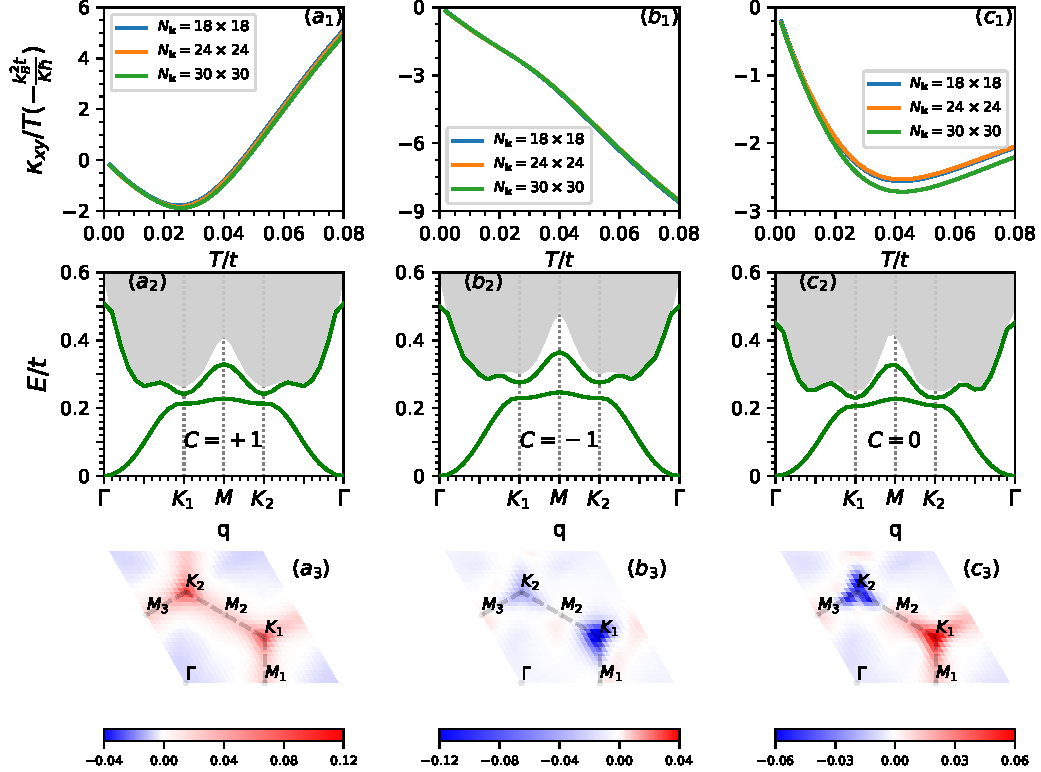
\includegraphics[width=1.0\textwidth]{ThermalHallWithTemperature}
\caption{Top: temperature dependence of the thermal Hall conductivity contributed by the acoustic band with different system sizes for the (a$_1$) topological phase with $C=1$, (b$_1$) topological phase with $C=-1$, and (c$_1$) trivial phase with $C=0$. Center: spin-1 excitation spectra along a high-symmetric path in the Brillouin zone with $N_\mathbf{k}=30\times30$ correspondingly. Bottom: Berry curvature in momentum space of the acoustic band with $N_\mathbf{k}=30\times30$ correspondingly. The parameters are (a) $t^\prime=0.29$, $U_B=1.2$, (b) $t^\prime=0.32$, $U_B=1.2$, and (c) $t^\prime=0.308$, $U_B=1.0$. Other parameters are fixed at $t=1.0$, $\phi=0.656$, $U_A=1.2$.}
\label{THWT}
\end{figure}

\par As has been discussed above, thermal Hall conductivity exhibits essentially different temperature dependence for topologically distinct phases. More prominent features are expected when the system undergoes a topological phase transition at a fixed temperature by varying the model parameters. In principle, the contributions from the optical band cannot be ignored in this case because of the gap closing at the transition point. Yet, these contributions cannot be faithfully computed due to the ill-defined Berry curvatures where the optical band touches the Stoner continuum. Therefore, we would ignore the optical band at first, present the data, and then discuss how it would modify the results. Fig. \ref{THWH}(a) replots the phase diagram of the model. Here, NFM denotes the non-ferromagnetic phase, FM denotes the trivial ferromagnetic phase, and TFM$^+$ (TFM$^-$) denotes the topological ferromagnetic phase with the Chern number $C=+1$ ($C=-1$). In the $\Delta U-t^\prime$ parameter space, we choose two paths marked by the green line and red line to compute the thermal Hall conductivity contributed by the acoustic band with a fixed temperature $T=0.08t$. The results are presented in Fig. \ref{THWH}(b) and Fig. \ref{THWH}(c), respectively. In Fig. \ref{THWH}(b), with the increase of $t^\prime$, the system undergoes a topological phase transition from TFM$^+$ phase to TFM$^-$ phase. Correspondingly, $\kappa_{xy}$ changes suddenly from a positive value ($\sim0.2$) to a negative value ($\sim-0.6$). In Fig. \ref{THWH}(c), with the increase of $t^\prime$, the system undergoes two successive topological phase transitions, the first from TFM$^+$ to FM, and the second from FM to TFM$^-$. Correspondingly, $\kappa_{xy}$ exhibits two successive jumps, the first from $\sim0.3$ to $\sim-0.2$, and the second from $\sim-0.2$ to $\sim-0.7$. When the contributions of the optical band come in, the observed discontinuous change of $\kappa_{xy}$ is expected to be softened. This is because the optical band possesses an opposite Chern number to the acoustic band, thus always cancels parts of the latter's contributions. At the transition point, the gap between the two bands vanishes and the cancelation reaches the maximum. As a result, the discontinuity weakens: a smooth curve is expected and the inflection point could indicate where the transition occurs.

\par In summary, by treating the itinerant magnons as canonical bosons, we calculate the thermal Hall conductivity of a flatband itinerant ferromagnet at low temperatures. This method is reliable when the optical band is separated from the acoustic band by an large enough energy gap. Although nonzero thermal Hall conductivity exists for all three topologically different phases, quite distinct behaviors are observed in their temperature dependences. By varying the model parameters, noticeable change of thermal Hall conductivity could be observed and be used to identify the topological phase transitions.

\begin{figure}
\centering
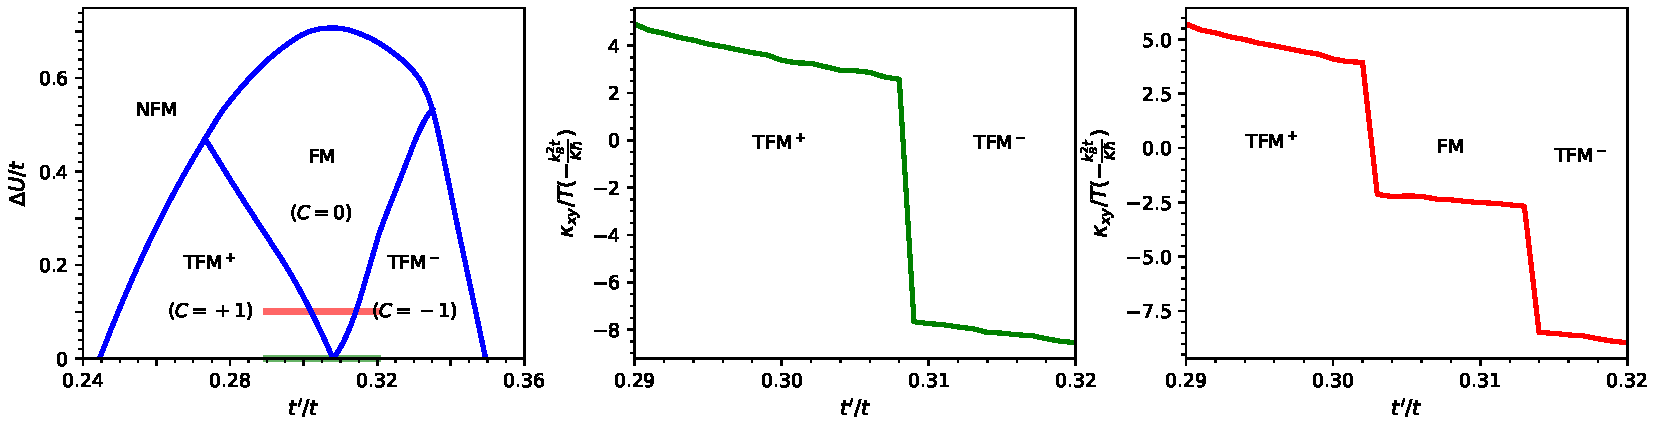
\includegraphics[width=1.0\textwidth]{ThermalHallWithHopping}
\caption{(a) Phase diagram of the model. Here, NFM denotes the non-ferromagnetic phase, FM denotes the trivial ferromagnetic phase, and TFM$^+$ (TFM$^-$) denotes the topological ferromagnetic phase with the Chern number $C=+1$ ($C=-1$). The green (red) solid line marks the parameters used in the subfigure (b) [(c)]. (b)-(c):  Thermal Hall conductivity contributed by the acoustic band versus the next-nearest-neighbor hopping amplitude $t^\prime$ with a fixed temperature $T=0.08t$.}
\label{THWH}
\end{figure}
\bibliography{reference}


\end{document}
